\documentclass{article}
\usepackage{graphicx}
\usepackage{amsmath}
\usepackage{amssymb}
\usepackage[margin=0.5 in]{geometry}
\usepackage{amsfonts}
\usepackage[shortlabels]{enumitem} 
\usepackage{amsthm}
\usepackage[dvipsnames]{xcolor}
\usepackage{thmtools}
\usepackage{stackengine}
\usepackage{float}
\usepackage{hyperref}
\usepackage{subcaption}
%\usepackage{movie15}
\usepackage{xcolor}
\usepackage{cancel}
\usepackage{hyperref}
\usepackage{verbatim}

\usepackage[framemethod=TikZ]{mdframed}
\mdfdefinestyle{mdbluebox}{%
	roundcorner = 10pt,
	linewidth=1pt,
	skipabove=12pt,1
	innertopmargin=12pt,
	innerbottommargin=9pt,
	skipbelow=2pt,
	linecolor=blue,
	%nobreak=true,
	backgroundcolor=TealBlue!5,
}
\declaretheoremstyle[
headfont=\sffamily\bfseries\color{blue},
mdframed={style=mdbluebox},
headpunct={\\[3pt]},
postheadspace={0pt}
]{thmbluebox}

\theoremstyle{definition} % bold + upright
\newtheorem{prob}{Problem}
\newtheorem{probe}{Extra Problem}
%\declaretheorem[style=thmbluebox,name=Theorem,numbered=no]{thm*}
\newtheorem*{sol}{Solution}

\title{Week of December 8 Report}
\author{Benjamin Campbell}
\date{December 10, 2025}

\newcommand{\ds}{\displaystyle} % force math styling

\newcommand{\sign}{\text{sign}}

\newcommand{\R}{\mathbb{R}} % reals
\newcommand{\Z}{\mathbb{Z}} % integers
\newcommand{\Q}{\mathbb{Q}} % rationals
\newcommand{\N}{\mathbb{N}} % naturals
\newcommand{\C}{\mathbb{C}} % complex

\newcommand{\supnorm}[1]{\left|\left|#1\right|\right|_\infty}


%% Linear algebra
\newcommand{\mat}[1]{\begin{bmatrix*}[r]#1\end{bmatrix*}}
\newcommand{\matc}[1]{\begin{bmatrix}#1\end{bmatrix}} % matrix
\newcommand{\Span}{\text{span}} % span
\newcommand{\Img}{\text{img}} % image
\newcommand{\Ker}{\text{ker}} % kernel
\newcommand{\Id}{\text{id}} % identity map
\newcommand{\Range}{\text{range}} % range
\newcommand{\Rref}{\text{rref}} % row reduced echelon form
\newcommand{\Rank}{\text{rank}} % rank
\newcommand{\Null}{\text{null}} % null space
\newcommand{\Nullity}{\text{nullity}} % nullity
\newcommand{\Proj}{\text{proj}} % projection
\newcommand{\Dim}{\text{dim}} % dimension

\stackMath
\newcommand\frightarrow{\scalebox{1}[.4]{$\rightarrow$}}
\newcommand\darrow[1][]{\mathrel{\stackon[1pt]{\stackanchor[1pt]{\frightarrow}{\frightarrow}}{\scriptstyle#1}}}

%% Topology
\newcommand{\Int}{int}
\newcommand{\Cl}{cl}
\newcommand{\norm}[1]{\left|\left|#1\right|\right|}

%% Calculus
\newcommand{\Length}{\text{length}} % length
\newcommand{\Area}{\text{area}} % area
\newcommand{\Vol}{\text{vol}} % volume
\newcommand{\Grad}{\text{grad}} % gradient
\newcommand{\Curl}{\text{curl}} % curl
\newcommand{\Div}{\text{div}} % divergence
\newcommand{\Conv}{\text{conv}} % convex hull 
\begin{document}

%% Classical Mechanics

\newcommand{\Teff}{T_{\text{eff}}}
\newcommand{\Ueff}{U_{\text{eff}}}
\newcommand{\Veff}{V_{\text{eff}}}

%% Chaos

\newcommand{\Per}{\text{Per}}

\maketitle

%\tableofcontents

\newpage

\section{Changes to the current algorithm}

Last week I had shown an improved algorithm for computing the current. This algorithm was meant to adjust the current to reflect driving forces from the voltage, to increase performance and fix issues with the original algorithm in which the calculated value did not reflect the definition of current as charge flow. Instead the original program simulated electrons moving through the system over some finite number of steps and simply counted the number that reached the other end. There are several issues with this approach, the most egregious being that as step number is increased, more electrons will reach the other end and thus current scaled with number of steps taken, an arbitrarily chosen value.

While my algorithm last week attempted to fix these issues by computing the current via the quantum tunneling resistances from the original paper in absence of Monte-Carlo sampling, it did not accurately predict the magnitude of the current. Thus this week I have implemented an entirely new algorithm for computing the current that attempts to use Monte-Carlo methods and the Metropolis algorithm alongside the tunneling resistances. The algorithm works according to the following steps:
\begin{enumerate}
\item If voltage is 0, return 0 since that will be the end result anyway - this saves a lot of computational time
\item Introduce num$_e$ electrons at random y-axis locations.
\item for each particle choose to move forward with Boltzman probability or backwards so sum is unity. This is done in the following way: find a typical tunneling distance given the location of the electron and use this to find the Boltzmann  factor associated with jumping twice this distance $e^{2d*\frac{V}{L_x}*q_e/k_BT}$ where $d$ is the tunneling distance, $L_x$ is the length of the device, $V$ is the voltage across the terminals, $q_e$ is the charge of a proton. Then the relative occupations at the site $d$ behind the current position and $d$ in front is $\frac{N_b}{N_f} = e^{e^{2d*\frac{V}{L_x}*q_e/k_BT}}$ so we take the probability of moving forward to be $p_f = \frac{1}{1+e^{e^{2d*\frac{V}{L_x}*q_e/k_BT}}}$ so that $\frac{p_f}{p_b} = e^{e^{2d*\frac{V}{L_x}*q_e/k_BT}}$ and $p_f + p_b = 1$.
\item Find the closest particle in the specified direction
\item Jump to that particle and record the resistance of the jump as $R_{\text{jump}} = R_t e^{d/\lambda}$ where $d$ is not the actual distance of the jump.
\item Update the position of the electrons
\item Repeat for each electron until all electrons have reached the end electrode
\item Sum up the resistances of the jumps. This is the resistance of a single path
\item Since electrons will preferably take paths with the least resistance we take a weighted average of the paths favoring the lowest resistances (currently I just count the lowest, but the change is easy). I tried taking a simple arithmetic mean but it seems that the resistances were ill-aligned with each other so when many electrons were sampled we got very jagged looking plots. Taking a weighted average helps to smooth the history so all of the plots shown take weighted averages.
\item Return current as $I = \frac{V}R$.
\end{enumerate}

Not only does this have fairly fast performance for num$_e \le 100$ but it provides curves that share a similar shape to the experimental data provided to me by Gloria. It also allows for electrons to move backwards if the voltage is too low which was not possible in the previous simulations.

\section{What the Current History looks like now}

\begin{center}
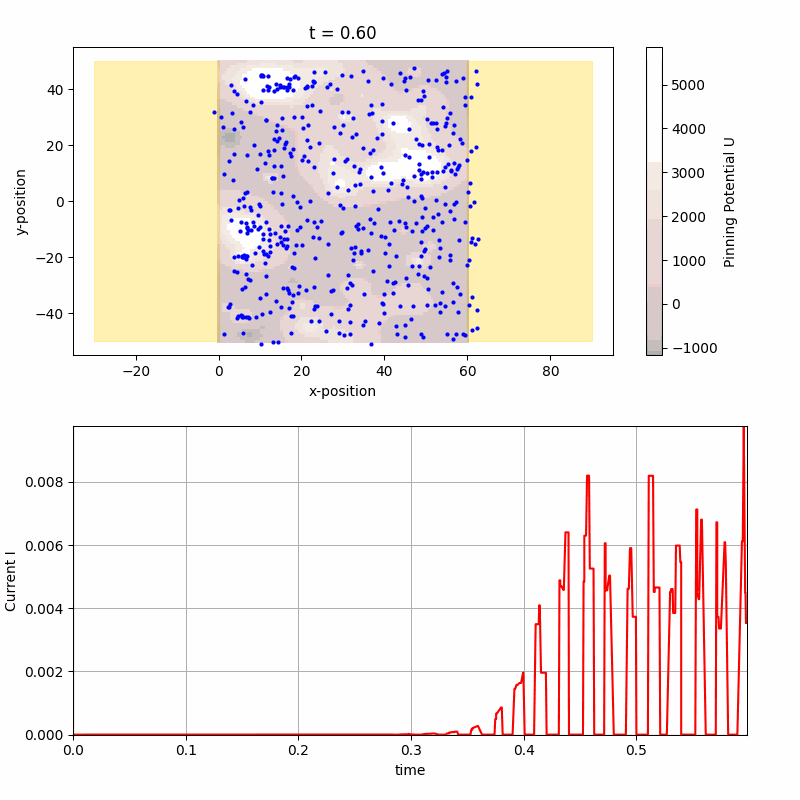
\includegraphics[width=0.9\textwidth]{20e-frame_499_delay-0.01s.png}
\end{center}

Above we show the current history when 20 electrons are sampled and below, when 100 electrons are sampled.

\begin{center}
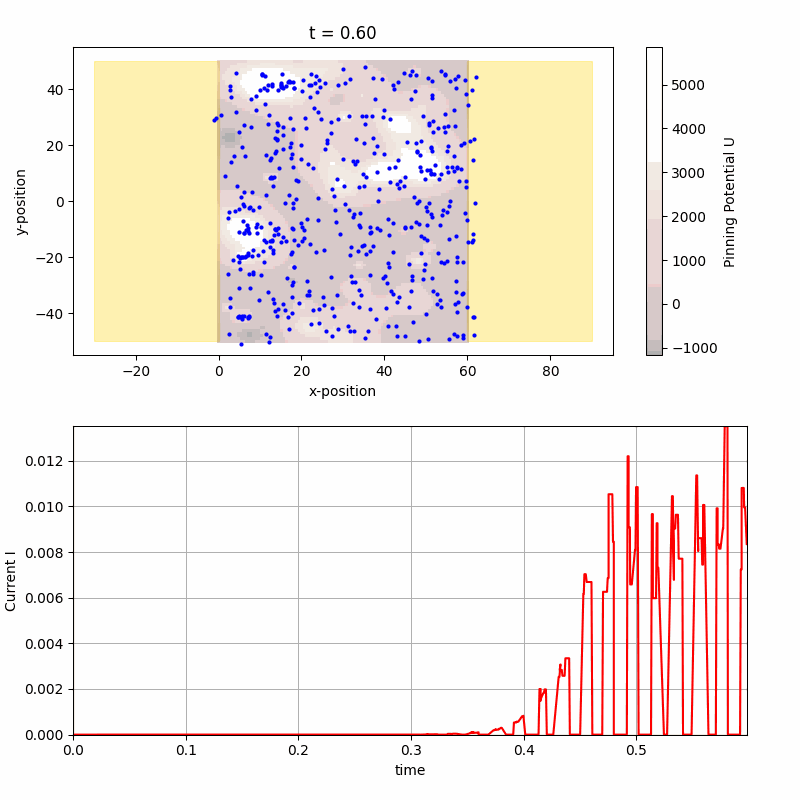
\includegraphics[width=0.9\textwidth]{100e-frame_499_delay-0.01s.png}
\end{center}

We see that there is very little difference in resolution so we may use $20$ electrons for efficiency.

\section{Changes in the current history as pinning potential magnitude changes}

\begin{figure}[H]
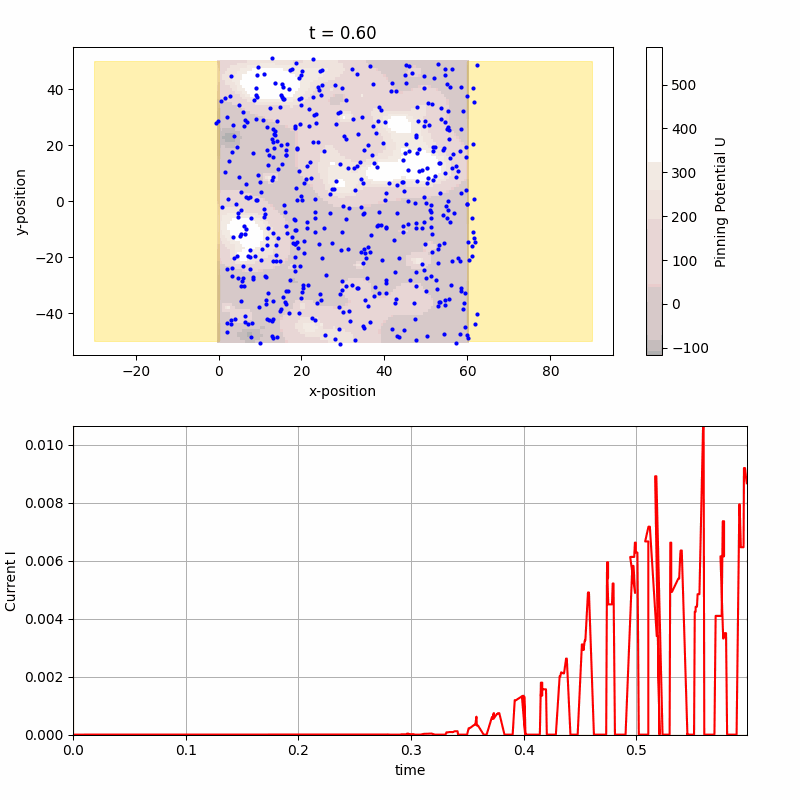
\includegraphics[width=0.3\textwidth]{last_frame_pin_div_10.png}
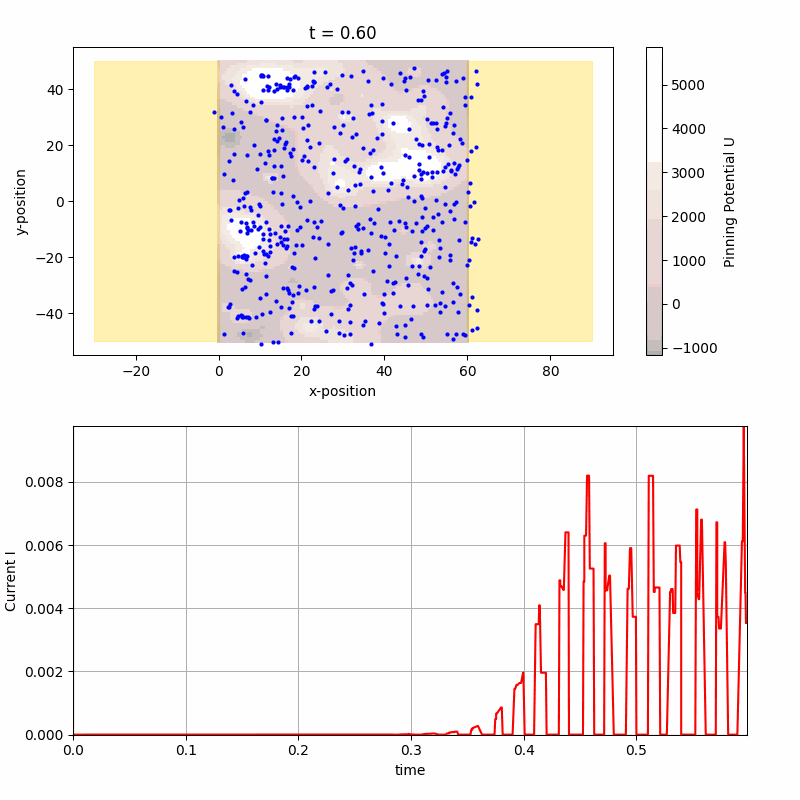
\includegraphics[width=0.3\textwidth]{20e-frame_499_delay-0.01s.png}
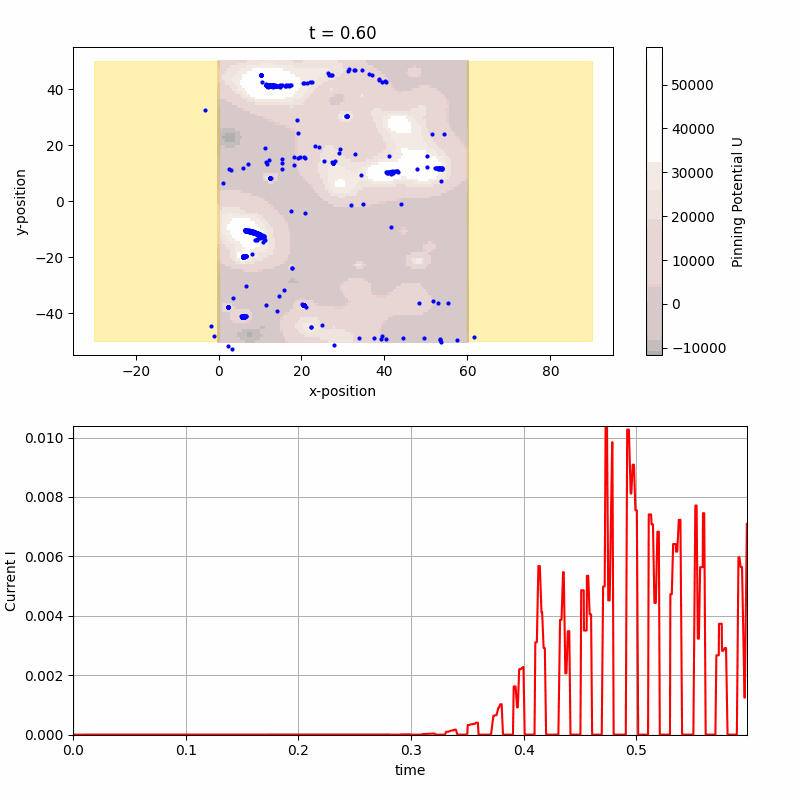
\includegraphics[width=0.3\textwidth]{last_frame_pin_mul_10.png}
\caption{From left to right we show the pinning potential increase 10 fold each time.}
\end{figure}

The pinning potential has a relatively mild effect on the current history. However, it seems that the higher the potential the more stable the paths will be in the long run since the particles become trapped in the potential wells. This is just a hypothesis though. We should test this over a longer time range. In particular pay attention to the particle positions in addition to the current graph for this section.

\section{Changes in the current history as Voltage changes}

\begin{figure}[H]
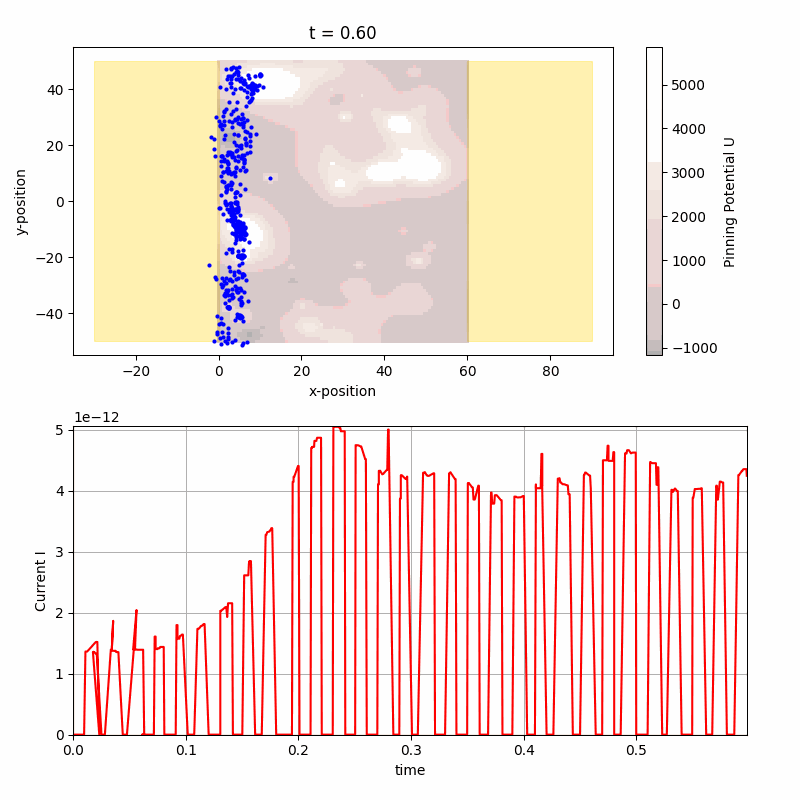
\includegraphics[width=0.3\textwidth]{last_frame_v-01.png}
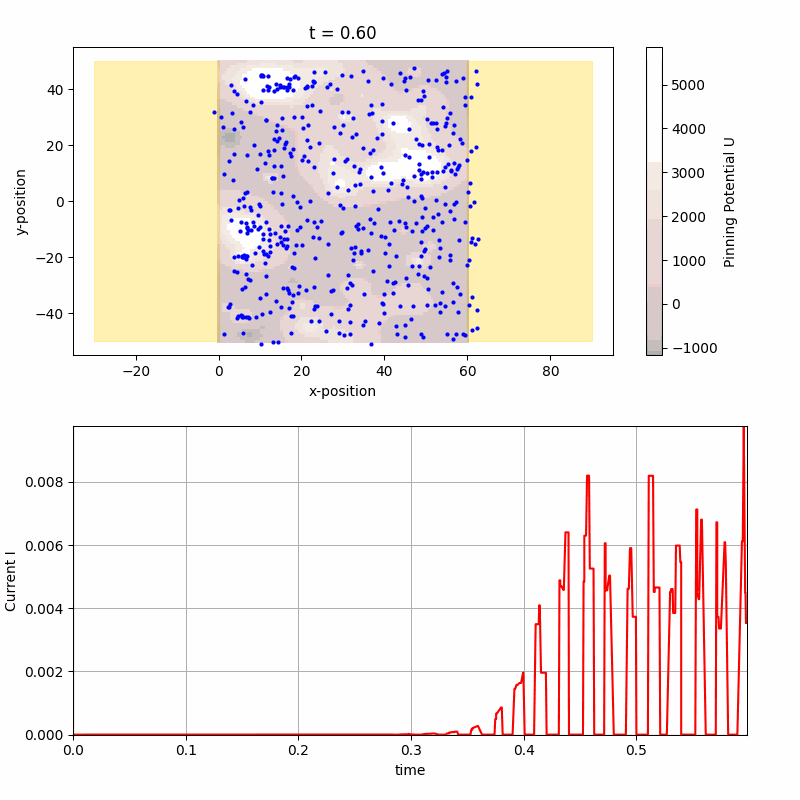
\includegraphics[width=0.3\textwidth]{20e-frame_499_delay-0.01s.png}
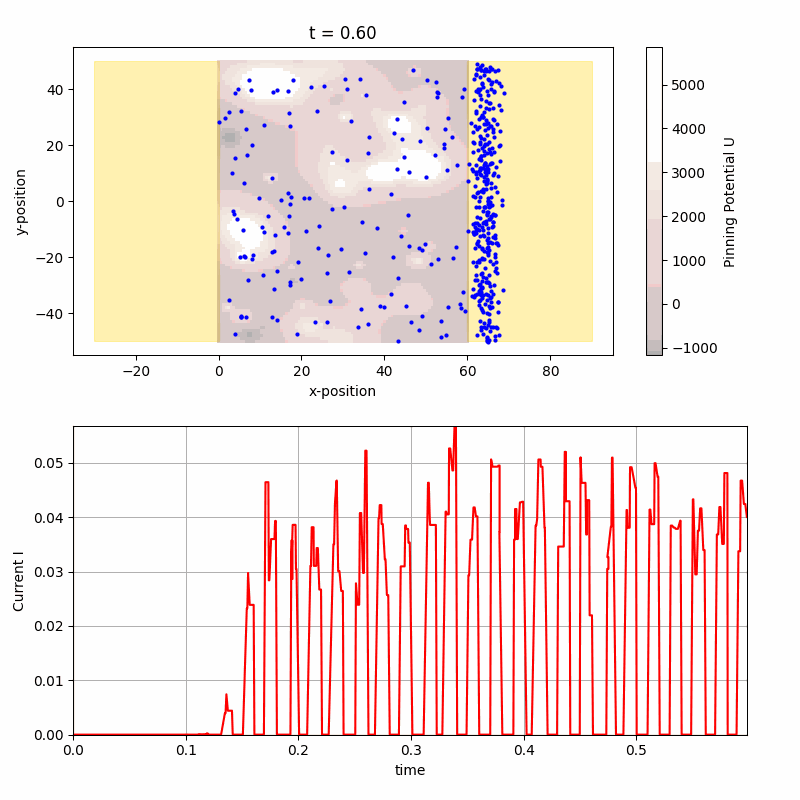
\includegraphics[width=0.3\textwidth]{last_frame_v-10.png}
\caption{From left to right we show the the voltage as $0.1,~3,~10$. Note that the scale in the left most figure is $\time 10^{-12}$ while the others are not.}
\end{figure}

Essentially voltage affects three things, the speed of the simulation, the maximal value of the current (which is also affected by the degree of completion) and the time at which switching occurs (if at all). Since there are pulses, the voltage must be enough to overcome any drift when the pulse is off. We see that this is not the case when the voltage is $0.1$ but is the case for the other two scenarios.


\section{effect of $\lambda$ (effective tunneling distance) on the current history}

\begin{figure}[H]
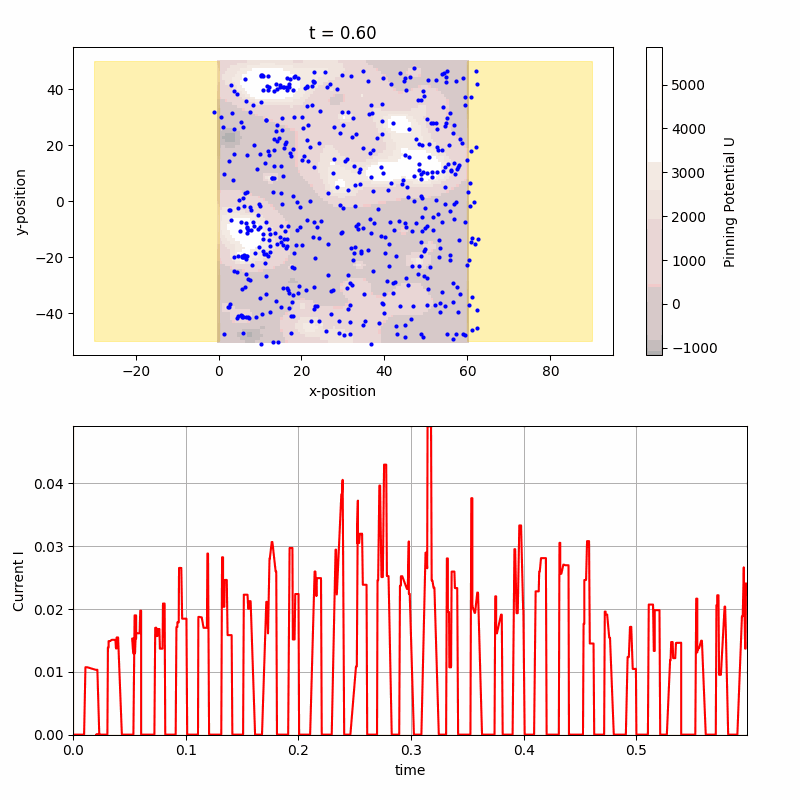
\includegraphics[width=0.3\textwidth]{last_frame_lam_10.png}
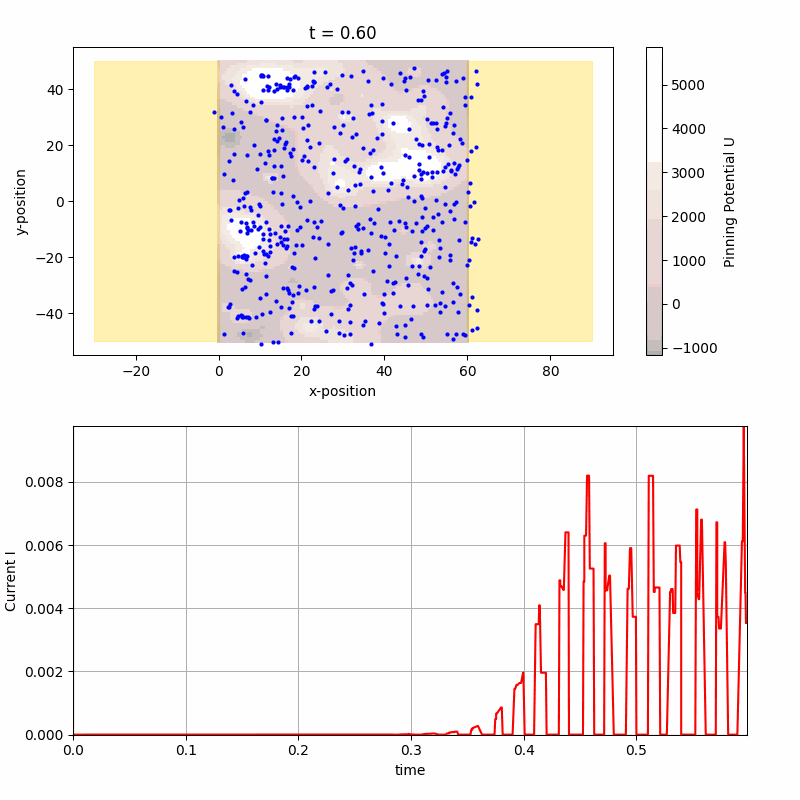
\includegraphics[width=0.3\textwidth]{20e-frame_499_delay-0.01s.png}
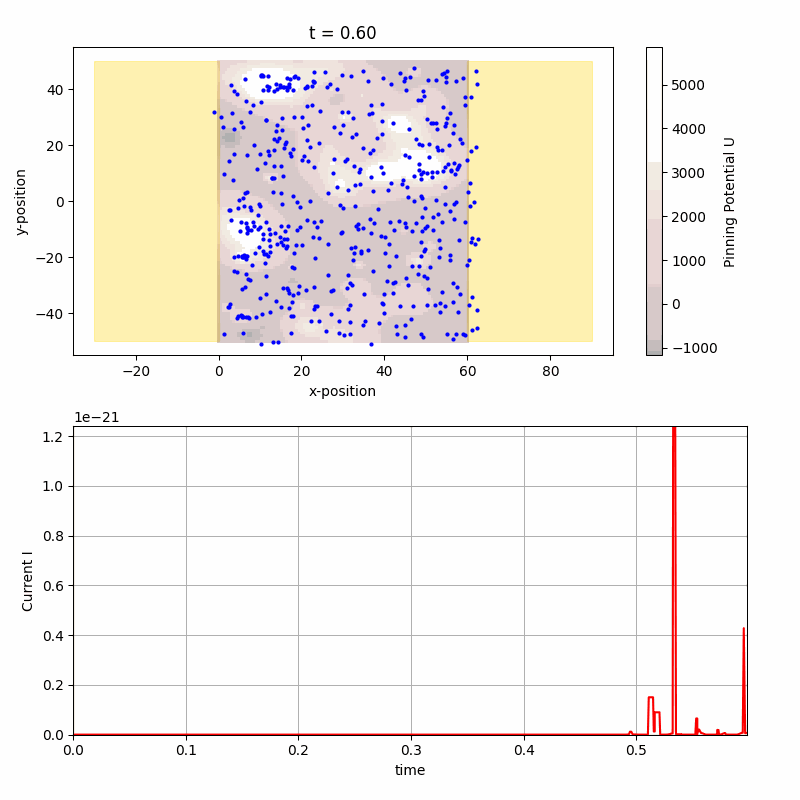
\includegraphics[width=0.3\textwidth]{last_frame_lam_01.png}
\caption{From left to right we show $\lambda = 0.1, 2, 10$.}
\end{figure}

We see clearly then that the desired choice of $\lambda$ is on the order of $1$. Our choice of $2$ works well.


\end{document}